% !TEX root=../master.tex

\chapter{Learning-based Object Re-identification}

\section{Background and Motivation}
One of the challenging aspects of performing a moving target handoff is ensuring, with enough confidence, that the handoff UAV has successfully identified the correct target before allowing the tracking UAV to leave.
In our current implementation, we only use classical feature tracking methods to determine the motion of the target and compare it with objects observed by the handoff vehicle.
Although we use vision-based features to track the target, we do not directly use visual information about the target as a descriptor to be used in comparing with other moving objects.
In the past few there have been increasingly impressive results in visual object classification and identification using deep neural networks (DNNs).
We conducted a preliminary study to see if we could utilize a deep neural network to encode and compare visual information about the target visually to objects observed by the handoff UAV. This appendix discusses the network architecture and training methods used, as well as some preliminary, but promising results.

\section{Implementation}
In order to demonstrate feasibility, we limited the scope of our study to focus specifically on person re-identification. There are many proposed methods for person re-identification. Many use only visual information \cite{} while some use recurrent networks to encode temporal information as well \cite{}.
We decided to base our architecture and methodology on the work done by Wang et al. in \cite{Wang2018} to create and train a network with a DenseNet architecture \cite{DenseNet}. The model is trained to take cropped bounding box images of people and embed them into clusters within a 128-dimensional vector space. The goal is to train the network in such a way that the cluster associated with each person is distinct and well-distanced (in an L2 norm sense) from embedded clusters of other people. This allows us to compare or identify people simply by measuring their L2 distance in the embedded vector space. Although we focused specifically on people for this study, we believe the extension to other classes of objects would be fairly straightforward, given sufficient data.

We trained the network using the Market-1501 dataset \cite{Market1501}, which consists of multiple cameras, allowing for multiple varied shots of the same people. Originally, we used the triplet loss function given in \cite{Wang2018}. The loss function is computed over a batch of $P$ people with $K$ unique images each. All images are embedded using the neural network and then their L2 distances are compared. For each image, the closest negative (non-matching embedding) and the furthest positive (matching embedding) are found and used to compute the total loss function, given by
\begin{equation}
    \ell = \sum_{p=1}^P \sum_{k=1}^K
            \ln \Bigg(1 + \exp\bigg(\big(
                m + (\text{closest positive})
                  - (\text{furthest negative})
            \big)\bigg)\Bigg)\;,
\end{equation}
where
\begin{equation}
    \text{closest positive} = \max_{a=1,\dots,K}D\left( \phi(x_p^k), \phi(x_p^a)\right);,
\end{equation}
\begin{equation}
    \text{furthest negative} = \min_{\substack{q=1,\dots,P \\ b=1,\dots,K \\ q\neq p}}
                                D\left( \phi(x_p^k), \phi(x_q^b)\right)\;,
\end{equation}
and $m$ represents a desired margin of separation between clusters.

Training using this loss function would decrease the total loss fairly well, but the network seemed to find a local minimum where it could minimize the loss simply by driving all embeddings toward the origin. In an effort to mitigate this challenge, we modified the loss function to minimize the ratio between the furthest positive and the closest negative. Accordingly, the loss function became
\begin{equation}
\label{eq:ratio_loss1}
    \ell = \sum_{p=1}^P \sum_{k=1}^K
            \frac{\text{furthest positive} + m}{\text{closest negative}} \;.
\end{equation}

Using this ratio-based loss removed any incentive to drive the embeddings toward the origin, but instead, allowed the network to spread out the clusters freely. Training with this loss had the advantage that we were able to train the network for longer without producing a degenerate solution and accordingly, the network learned how to more accurately represent detailed information. It was also quite a bit faster than the original loss function, providing a speed increase of about 20\%.

The main disadvantage to using this loss function is that it made the distances between an image and it's closest positive inconsistent across different people. This property is undesirable because it makes it difficult to infer whether or not two images match purely based on the L2 distance. Some matching images would be spaced 1 unit apart and others would be spaced 15-20 units apart.

In order to overcome this challenge, we reformed the loss function again to include a term that would penalize large distances between positive examples. The loss function became
\begin{equation}
\label{eq:ratio_loss2}
    \ell = \sum_{p=1}^P \sum_{k=1}^K
            \frac{\text{furthest positive} + m}{\text{closest negative}} + k(\text{furthest positive})\;,
\end{equation}
where $k$ is a scaling constant. We used a value of 0.1 for $k$.

We continued to train the previously trained network using this new loss function, hoping that it would maintain its understanding of how to group unique identities, but also learn to condense those embeddings to minimize the distance between positive examples. In general, the distances did decrease and the variability in distances within clusters was reduced, although not totally eliminated. Determining an effective way to allow the network to spread clusters out freely in a more consistent manner is a topic for future research and development.


\section{Results}

We trained the first ratio loss function given in Equation \eqref{eq:ratio_loss1} for about 13,000 iterations after which we switched to the second ratio loss given in \eqref{eq:ratio_loss2}. We continued training for another 5000 iterations and were able to obtain fairly good results. The network was able to maintain the accuracy that had been learned by the initial loss function, but also learned to embed positive examples closer together, bringing the max distance down from about 20 to 5.

In order to evaluate the progress of the network, we used a qaulitative measure of accuracy. Periodically, we sampled a batch of 20 people, each with 5 images, from the test dataset. We then calculated the embeddings of each image and the distances between all images. We randomly selected an image and displayed the 5 nearest images and their distances. Ideally, we would expect the chosen image and its 4 nearest embeddings to have the same identity and the 5th to be another person with a distance at least the desired margin further than the furthest positive example. Below we give some qaulitative results and our observations regarding the network's performance.

The network was usually fairly confident at re-identifying people with bright colors or distinct patterns such as in Figures 1-4.
\begin{figure}[H]
\label{fig:bright1}
        \centering 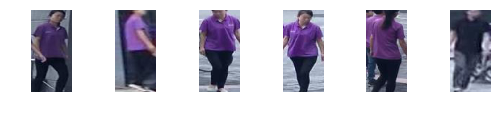
\includegraphics[width=0.8\columnwidth]{figures/person_reid/example7_confident.png}
        \caption{Example of bright clothing.}
\end{figure}

\begin{figure}[H]
\label{fig:bright2}
    \centering 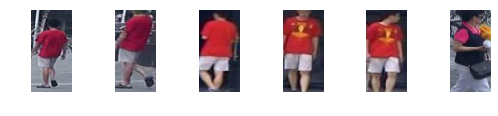
\includegraphics[width=0.8\columnwidth]{figures/person_reid/example8_confident.png}
    \caption{Another example of bright clothing.}
\end{figure}

\begin{figure}[H]
\label{fig:pattern1}
    \centering 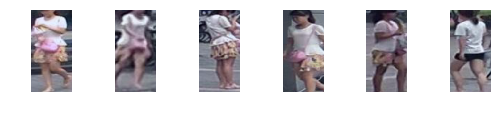
\includegraphics[width=0.8\columnwidth]{figures/person_reid/example4_perfect.png}
    \caption{Example of unique patterned clothing.}
\end{figure}

\begin{figure}[H]
\label{fig:pattern2}
    \centering 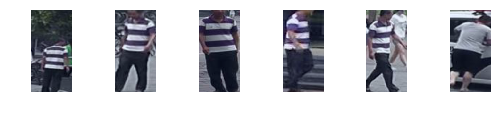
\includegraphics[width=0.8\columnwidth]{figures/person_reid/example12_pattern.png}
    \caption{Another example of patterned clothing.}
\end{figure}

It also performed surprisingly well in some difficult situations, such as when two people are similarly dressed, when the lighting varied between cameras, or when the same person is seen in multiple contexts (Figures 5-8).

\begin{figure}[H]
    \centering 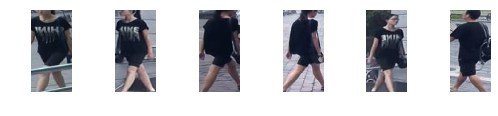
\includegraphics[width=0.8\columnwidth]{figures/person_reid/example11_accurate_despite_similarities.png}
    \caption{Successful classification despite there being two similarly dressed people.}
\end{figure}

\begin{figure}[H]
    \centering 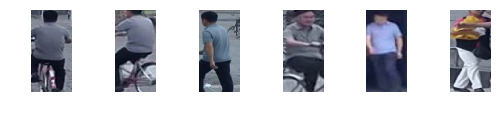
\includegraphics[width=0.8\columnwidth]{figures/person_reid/example8_different_context.png}
    \caption{Successful classification in varied lighting.}
\end{figure}

\begin{figure}[H]
    \centering 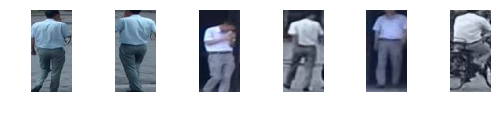
\includegraphics[width=0.8\columnwidth]{figures/person_reid/example2_lighting.png}
    \caption{Another example of successful classification in varied lighting.}
\end{figure}

\begin{figure}[H]
    \centering 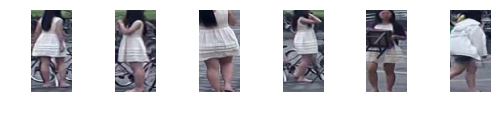
\includegraphics[width=0.8\columnwidth]{figures/person_reid/example6_different_context.png}
    \caption{Successful classification in varied contexts (the woman is carrying furniture and wearing a cardigan in the 5th image).}
\end{figure}

Often, even the failure cases were reasonable, such as two people that had similar clothing, scenes with common prominent features, or specific viewpoints that made classification difficult (Figures 9-12).

\begin{figure}[H]
    \centering 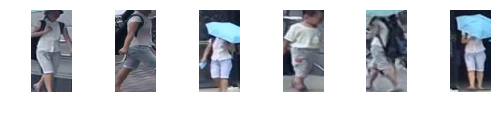
\includegraphics[width=0.8\columnwidth]{figures/person_reid/example1_similar.png}
    \caption{Incorrect classification of 4th image - similar clothing.}
\end{figure}

\begin{figure}[H]
    \centering 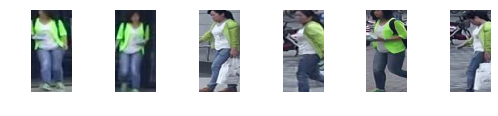
\includegraphics[width=0.8\columnwidth]{figures/person_reid/example3_similar.png}
    \caption{Incorrect classification of 3rd and 4th images - similar clothing.}
\end{figure}

\begin{figure}[H]
    \centering 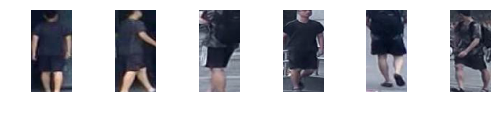
\includegraphics[width=0.8\columnwidth]{figures/person_reid/example5_reasonable_mistake.png}
    \caption{Incorrect classification of 3rd, 5th, and 6th images - similar clothing.}
\end{figure}

\begin{figure}[H]
    \centering 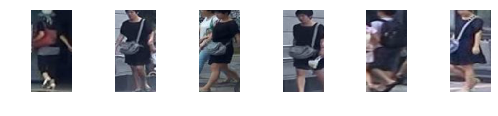
\includegraphics[width=0.8\columnwidth]{figures/person_reid/example9_no_matches.png}
    \caption{Incorrect classification of all images - grey undershirt mistaken as grey handbag.}
\end{figure}

Interestingly enough, it even seemed as though the network has some form of a bike detector, as seen in the failure mode of Figure 13.

\begin{figure}[H]
    \centering 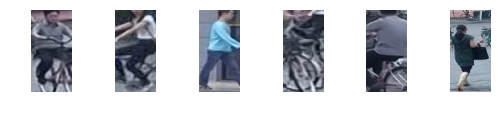
\includegraphics[width=0.8\columnwidth]{figures/person_reid/example10_bike_detector.png}
    \caption{Incorrect classification of 2nd, 3rd, 4th, and 6th images - seems to have been looking for bikes, at least partially.}
\end{figure}


\section{Conclusions}
With more training and some improvements in the loss function, we propose that using this or a similar method of training a neural network could prove useful in classifying and re-identifying objects based on visual information. Such a network would be especially useful in the case of the moving target handoff problem where the tracking vehicle could simply send the 128-dimensional embedding of the target object, allowing the handoff vehicle to compare the L2 embedding distance between the target and moving objects in its field of view. Not only does this provide a means of comparing valuable visual information, but it can also be done without needing to directly pass large image files between the vehicles. With some improvemens and increased reliability, this would provide a useful tool to take advantage of rich visual information that is currently not being utilized in our moving target handoff solution.
